
\subsection{{\idletime}が一般の場合}
\label{subsec:LineDifferentTimelimit}

全点の{\idletime}が等しい場合は
どの頂点も複数の巡査の協力で警備する必要がないため単純になっていたが,
{\idletime}が一般の場合は,
頂点を複数の巡査が交代で訪問して警備する必要がある場合が存在する.
%
図\ref{tikz:multiAgentExample2}(左)の例では,
中央の{\idletime}の短い2つの頂点を
2人の巡査が交互に訪問しており,
また,全点の{\idletime}が等しい場合と異なり
各巡査の最適な運行はなんらかの区間の往復であるとは限らないことも分かる.


また,
% \red{左から巡査の動きを決定できるのではないか?しかし,…
% ({\idletime}ぴったりの周期の場合についてのみ反例を作る?}
この例では左の巡査は左端の点を{\idletime}$10$ちょうどごとに訪問しているが,
左端の点の{\idletime}から順に巡査の運行を決定することも難しい次のような例が存在する.
図\ref{tikz:multiAgentExample2}(中央)の例では
{\idletime}$8$の左端の点をあえてより短い$6$ごとに訪問することで全点を警邏できるが,
同じグラフについて,
図\ref{tikz:multiAgentExample2}(右)のように左の巡査が
左端の点の{\idletime}ぎりぎりの時間まで右の方へ動き頂点をなるべく多くの時間訪問して左端へ帰る運行を選ぶと
右の巡査がどのような動き方をしても訪問間隔が{\idletime}を超え警備できない頂点が生まれてしまう.



\begin{figure}[h]
  \centering
  \begin{tabular}{ccc}

  \begin{minipage}{0.32\hsize}
    \centering
    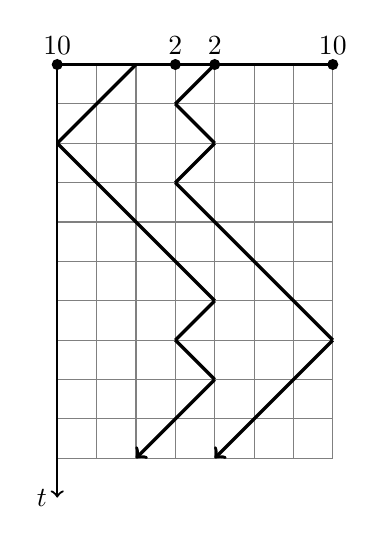
\begin{tikzpicture}
      \draw [help lines,thin,step=5mm] (0,-5.0) grid (3.5,0);
      \draw[thick] (0,0) -- (3.5,0) node [below] {};
      \draw[thick, ->] (0,0) -- (0,-5.5) node [left] {$t$};

      \fill ( 0   , 0) coordinate (c1) circle (2pt) node [above] {10};
      \fill ( 1.5 , 0) coordinate (c2) circle (2pt) node [above] {2};
      \fill ( 2.0 , 0) coordinate (c3) circle (2pt) node [above] {2};
      \fill ( 3.5 , 0) coordinate (c5) circle (2pt) node [above] {10};

      \draw[very thick,- ] ( 1.0, 0  )--(   0,-1.0);
      \draw[very thick,- ] (   0,-1.0)--( 2.0,-3.0);
      \draw[very thick,- ] ( 2.0,-3.0)--( 1.5,-3.5);
      \draw[very thick,- ] ( 1.5,-3.5)--( 2.0,-4.0);
      \draw[very thick,->] ( 2.0,-4.0)--( 1.0,-5.0);

      \draw[very thick,- ] ( 2.0, 0  )--( 1.5,-0.5);
      \draw[very thick,- ] ( 1.5,-0.5)--( 2.0,-1.0);
      \draw[very thick,- ] ( 2.0,-1.0)--( 1.5,-1.5);
      \draw[very thick,- ] ( 1.5,-1.5)--( 3.5,-3.5);
      \draw[very thick,->] ( 3.5,-3.5)--( 2.0,-5.0);
    \end{tikzpicture}
  \end{minipage}

  \begin{minipage}{0.32\hsize}
    \centering
    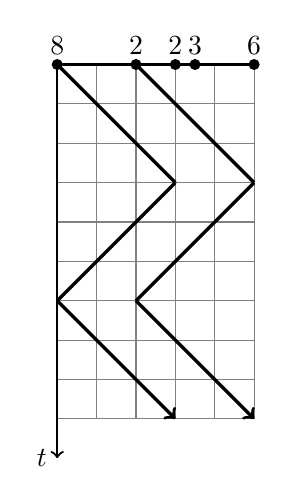
\begin{tikzpicture}
      \draw [help lines,thin,step=5mm] (0,-4.5) grid (2.5,0);
      \draw[thick] (0,0) -- (2.5,0) node [below] {};
      \draw[thick, ->] (0,0) -- (0,-5) node [left] {$t$};

      \fill ( 0   , 0) coordinate (c1) circle (2pt) node [above] {8};
      \fill ( 1   , 0) coordinate (c2) circle (2pt) node [above] {2};
      \fill ( 1.5 , 0) coordinate (c3) circle (2pt) node [above] {2};
      \fill ( 1.75, 0) coordinate (c4) circle (2pt) node [above] {3};
      \fill ( 2.5 , 0) coordinate (c5) circle (2pt) node [above] {6};

      % \draw[very thick,red,<->] (1.75,-0.75)--(1.75,-2.25);

      \draw[very thick,- ] ( 0  , 0  )--( 1.5,-1.5);
      \draw[very thick,- ] ( 1.5,-1.5)--( 0  ,-3  );
      \draw[very thick,->] ( 0  ,-3  )--( 1.5,-4.5);
      \draw[very thick,- ] ( 1  , 0  )--( 2.5,-1.5);
      \draw[very thick,- ] ( 2.5,-1.5)--( 1  ,-3  );
      \draw[very thick,->] ( 1  ,-3  )--( 2.5,-4.5);
    \end{tikzpicture}
  \end{minipage}

  \begin{minipage}{0.32\hsize}
    \centering
    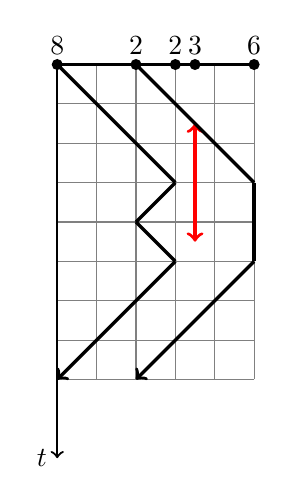
\begin{tikzpicture}
      \draw [help lines,thin,step=5mm] (0,-4) grid (2.5,0);
      \draw[thick] (0,0) -- (2.5,0) node [below] {};
      \draw[thick, ->] (0,0) -- (0,-5) node [left] {$t$};

      \fill ( 0   , 0) coordinate (c1) circle (2pt) node [above] {8};
      \fill ( 1   , 0) coordinate (c2) circle (2pt) node [above] {2};
      \fill ( 1.5 , 0) coordinate (c3) circle (2pt) node [above] {2};
      \fill ( 1.75, 0) coordinate (c4) circle (2pt) node [above] {3};
      \fill ( 2.5 , 0) coordinate (c5) circle (2pt) node [above] {6};

      \draw[very thick,red,<->] (1.75,-0.75)--(1.75,-2.25);

      \draw[very thick,- ] ( 0  , 0  )--( 1.5,-1.5);
      \draw[very thick,- ] ( 1.5,-1.5)--( 1  ,-2  );
      \draw[very thick,- ] ( 1  ,-2  )--( 1.5,-2.5);
      \draw[very thick,->] ( 1.5,-2.5)--( 0  ,-4  );

      \draw[very thick,- ] ( 1  , 0  )--( 2.5,-1.5);
      \draw[very thick,- ] ( 2.5,-1.5)--( 2.5,-2.5);
      \draw[very thick,->] ( 2.5,-2.5)--( 1  ,-4  );
    \end{tikzpicture}
  \end{minipage}

  \end{tabular}
  \caption{巡査の協力が必要な例.
    横軸を頂点の座標,縦軸を時刻として巡査の軌跡を表す.
    点の上の数値は{\idletime}を表す.
    \label{tikz:multiAgentExample2}}
\end{figure}




これらの例は,協力が発生する場合巡査の運行を個別に決定するのは難しいということを示唆している.
しかしながら,この{\idletime}が一般の場合でのLine上の{\patProb}の困難性を示すこともできなかった.
そこで,{\idletime}より短い間隔で点を訪問しうることで運行の決定を複雑になる例が存在したことを踏まえて,
1章で定義した時刻指定協力警邏判定問題を考える.




\begin{defi}
  $X \subset \Zset \times \Nset$とする.
  任意の$(t, x), (t', x') \in X$が
  $|t - t'| \geq |x - x'|$
  を満たすとき,$X$は運行可能であるという.
\end{defi}


任意の運行可能な集合$X$に対して,
Line上の巡査の運行$a$であって,
$X$のすべての元$(t, x)$に対して$a(t) = x$を満たすものが存在することは簡単に示すことができる.
これにより,
グラフがLineの場合の時刻指定協力警邏判定問題は次のようにも記述できる.

\begin{timeSpecifiedProblemOnLine}
  正の整数$m$(巡査の人数を表す)
  と自然数の組$(q_i, r_i, x_i)_{ i \in \{ 1, \ldots, n \} }$が与えられる.
  集合
  $\{ (q_i k + r_i, x_i) \mid i \in \{1, \ldots, n\}, k \in \Zset \}$
  を$m$個以下の運行可能な集合に分割できるか判定せよ.
\end{timeSpecifiedProblemOnLine}


% これを解くために次の副問題を考える.

% 1周期分だけ取り出して分割可能であることと元のXが分割可能であることが一致することを説明し
% アルゴリズムでは無限集合の周期的な分割を与えてYesかNoを答える
この問題では,
$X := \{ (q_i k + r_i, x_i) \mid i \in \{1, \ldots, n\}, k \in \Zset \}$
という無限集合の分割が可能か判定する必要があるが,
実際には$X$の点は時刻(組$(t, x) \in X$の第1要素)方向に周期的に並んでいるため,
その1周期分の有限部分集合を以下に定義する「周期的に運行可能な集合」に分割できるかどうかさえ
判定すればよい.

\red{理由を説明}

\begin{defi}
  $T$を正の整数,$X \subset \Zset \times \Nset$を有限集合とする.
  任意の$(t, x), (t', x') \in X$が
  $|t - t'| \geq |x - x'|$
  かつ
  $|t + T - t'| \geq |x - x'|$
  を満たすとき,$X$は周期$T$で繰り返し運行可能であるという.
\end{defi}


% \begin{timeSpecifiedProblemOnLineSubProb}
%   正の整数$m$
%   と自然数の組$(q_i, r_i, x_i)_{ i \in \{ 1, \ldots, n \} }$が与えられる.
%   集合
%   $X := \{ (q_i k + r_i, x_i) \mid i \in \{1, \ldots, n\}, k \in \Zset \}$
%   を$m$個以下の運行可能な集合に分割できるか判定し,
%   できるならば,
%   $T := lcm( q_1, \ldots, q_n )$とし,
%   有限集合
%   $\{ (t, x) \in X \mid 0 \leq t < T \}$
%   を周期$T$で繰り返し運行可能な$m$個以下の集合に分割せよ.
% \end{timeSpecifiedProblemOnLineSubProb}

% 明らかに時刻指定線分警邏問題は副問題に帰着できる.
% この副問題では上記のような$X$の分割が可能である場合には
% 必ず周期的な分割が存在することを主張している.
% % その1周期分の有限部分集合
% % $\{ (t, x) \in X \mid 0 \leq t < T \}$
% % の分割を与えることにより$X$全体の分割が可能であることを主張している.
% 実際に,この副問題は以下の貪欲アルゴリズムによって解くことができる.



% \begin{figure}[h]
%   \centering
%   \begin{tikzpicture}
%     \fill [fill=lightgray]
%       (1.5, -2)--(3.5,0)--(4,0)--(4,-4)--(3.5,-4)--(1.5, -2);
%     \draw[thick, ->] (0,0) -- (4.5, 0) node [below] {$x$};
%     \draw[thick, ->] (0,0) -- (0,-4) node [left] {$t$};

%     \fill ( 1.5,-2) coordinate (a) circle (2pt) node [left] {$(\alpha, \beta)$};

%     \node (L) at (1,-1.25) {$L(\alpha, \beta)$};
%     \node (R) at (3,-2) {$R(\alpha, \beta)$};
%   \end{tikzpicture}
%   \caption{$L(\alpha, \beta)$ と $R(\alpha, \beta)$ の定義 \label{tikz:defLR}}
% \end{figure}


\begin{greedyAlgorithmForTimeSpecifiedProblemOnLine}
  入力を$(m, (q_i, r_i, x_i)_{ i \in \{ 1, \ldots, n \} })$とする.
  始めに
  $T := lcm(q_1, \ldots, q_n)$,
  $X := \{ (q_i k + r_i, x_i) \mid i \in \{1, \ldots, n\}, k \in \Zset \}$,
  $L((\alpha, \beta)) := \{(t, x) \mid x - \beta \leq |t - \alpha| \}$と記号を定義する.

  まず$X$の部分集合$S := \{ (x, t) \in X \mid -T \leq t < 2T \}$を求める.
  初期値を$\mathcal{B} = \{\}$, $B_0 = S$, $B' = S$, $i = 0$とし,
  $B_i \neq \emptyset$である限り1.から4.を繰り返す.
  \begin{enumerate}
    \item $i \gets i + 1$, 
    \item $B_i \gets B' \cap \left( \bigcap_{p \in B'} L(p) \right)$, 
    \item $B' \gets B' \setminus B_i$, 
    \item $\mathcal{B} \gets \mathcal{B} \cup \{ B_i \}$.
  \end{enumerate}

  $|\mathcal{B}| > m$ならば分割不可能と答え,
  そうでないときは分割可能と答えたうえで,
  $\mathcal{B}$の各元を時刻方向に$[0, T)$に制限したもの
  $\mathcal{C} := \{ \{ (t, x) \in B \mid 0 \leq t < T \} \mid B \in \mathcal{B} \}$
  を出力して終了する.
\end{greedyAlgorithmForTimeSpecifiedProblemOnLine}

% 副問題は主問題の判定を行いさらに繰り返し運行可能分割を求める問題なので,
% 主問題の判定ができていることをここで説明する必要がある.
この貪欲アルゴリズムが
\begin{itemize}
  \item 分割不可能と答えるとき,
    $X$も$m$個の運行可能な集合に分割することはできない.
    実際,
    $X$が$m$個の運行可能な集合に分割できるとき,
    $S := \{ (x, t) \in X \mid -T \leq t < 2T \}$
    は$X$の部分集合であるから$m$個の運行可能な集合に分割できるが,
    その場合は貪欲アルゴリズムは必ず$m$個の運行可能な集合への分割を答える.
    これは次の理由による.
    Lineにおいては順序保存運行の存在と同様に,
    $S$が$m$個の運行可能な集合へ分割可能ならば
    $S$の$m$個の運行可能な集合への分割であって順序保存なものが存在する.
    ここで,分割$\mathcal{B'} = \{ B'_1, \ldots, B'_m \}$が順序保存であるとは,
    対応する運行$(b_1, \ldots, b_m)$が順序保存運行になることである.
    貪欲アルゴリズム中で得られる$S$の分割$\mathcal{B} = \{ B_1, \ldots, B_m \}$は
    任意の順序保存な$S$の分割を選び$\mathcal{B'} = \{ B'_1, \ldots, B'_m \}$と整数$k$に対し,
    $\bigcup_{1 \leq i \leq k} B'_i \subseteq \bigcup_{1 \leq i \leq k} B_i$
    を満たしており,これにより
    $S$が$m$個の運行可能な集合へ分割可能ならば
    貪欲アルゴリズムは必ず$m$個の運行可能な集合への分割を答えることが分かる.
  \item 分割可能と答えるとき,
    $X$も$m$個の運行可能な集合に分割することができる.
    実際,
    分割可能と答えるときには分割$\mathcal{C}$を出力するが,
    $\mathcal{C}$の各元$C$は
    周期$T$で繰り返し運行可能な集合である.
    これは,途中の各$B \in \mathcal{B}$が$L$の定義から運行可能集合となっており,
    $B$の$[-T, 2T)$の範囲が運行可能であれば$[0, T)$の範囲は
    定義から周期$T$で繰り返し運行可能となるためである.

    集合
    $X := \{ (q_i k + r_i, x_i) \mid i \in \{1, \ldots, n\}, k \in \Zset \}$
    の分割$\mathcal{A} = \{ A_1, \ldots, A_m \}$は次のように構成すればよい.
    $k \in \Zset$に対して,$X$の部分集合
    $\{ (t, x) \in X \mid kT \leq t < (k + 1)T \}$
    を$\mathcal{C}$の分割の仕方で分割したものを$\{ C_{k1}, \ldots, C_{km} \}$とする.
    $A_i := \bigcup_{k \in \Zset} C_{ki}$と定義すると,
    $C_{ki}$が周期$T$で繰り返し運行可能な集合であるから,
    $A_i$は運行可能な集合となる.
    % $\mathcal{A}$は$X$を$m$個の運行可能な集合へ分割したものとなっている.
\end{itemize}
以上より,貪欲アルゴリズムは副問題を解く.





% 三角形領域$R(t_a, x_a)$は,
% 時刻$t_a$に$x_a$に存在する巡査が存在し得ない位置と時刻の組の集合のうち
% $x_a$より右側の領域を表している($|x - x_a| / |t - t_a| > 1$かつ$x_a < x$).
% 訪問しなければならない位置と時刻の組の集合$X$に対して,
% $\dbigcap_{a \in X} L(a)$は
% 一番左の巡査の存在可能領域を表す(補題**).



% 本節で示すのは以下の定理である.
% \begin{theo}
%   \label{lemm:LineExactFinite}
%   グラフの形状がLineのとき,
%   時刻指定{\patProb}は,
%   「最右運行」で巡査の運行を左端から順に決定する\red{(←手順が未定義)}ことで
%   全点警邏可能か判定できる.
%   % \red{
%   %   指定時刻が有限個ならその個数の多項式時間で判定できる、とかにする?
%   %   入力が周期と剰余なら$O(*)$で計算できる、とかに?
%   % }
% \end{theo}


% \begin{lemm}
%   \label{lemm:leftmostAgentExistableTerrain}
%   $X$を訪問しなければならない位置と時刻の組の集合とする.
%   このとき,
%   順序保存運行において一番左の巡査$s$の軌跡は
%   $\bigcap_{a \in X} L(a)$に含まれる.
% \end{lemm}

% \begin{proof}
%   巡査$s$の軌跡に$\bigcup_{a \in X} R(a)$の点$b = (t_b, x_b)$が含まれるとすると,
%   ある$a = (t_a, x_a) \in X$が存在して$b \in R(a)$となる.
%   巡査の速さは1以下なので時刻$t_a$における巡査$s$の位置$x$は
%   $|x_b - x| \leq |t_b - t_a|$を満たすが,
%   $b \in R(a)$より$x_b - x_a > |t_b - t_a|$なので
%   $x_b - x \leq |x_b - x| < x_b - x_a$,
%   すなわち$x_a < x$となる.
%   $x_a < x$より$x_a$を警備する$s$より左の巡査が必要になり矛盾する.
%   よって,$s$の軌跡は$\bigcup_{a \in X} R(a)$の点を含まない.
% \end{proof}

% これにより次がいえる.

% \begin{lemm}
%   \label{lemm:LineExactFinite}
%   グラフ$G$がLine,指定時刻全体が$X$のときの時刻指定{\patProb}において,
%   $m$人の巡査により$G$を警邏可能であるとき,
%   $m$人の巡査のうち
%   $1$人の巡査が$X$に対する最右運行であるような運行により$G$を警邏できる.
% \end{lemm}

% \begin{proof}
%   指定時刻の集合を$X$とする.
%   $G$は$m$人の巡査により警邏可能であるので,
%   2章始めの議論により$G$を警邏する$m$人の巡査による順序保存運行が存在する.
%   このような運行を任意に一つ選び$A = (a_1, \ldots, a_m)$とする.
%   補題\ref{lemm:leftmostAgentExistableTerrain}より
%   $A$における一番左の巡査の運行$a_1$の軌跡は
%   $\bigcap_{a \in X} L(a)$に含まれる.
%   $\bigcap_{a \in X} L(a)$に含まれる$X$の点は$b(X)$上に存在するので
%   $a_1$の軌跡に含まれる$X$の点は$b(X)$に含まれる.
%   一方,$b(X)$は傾きが$\pm 1$の線分からなる連続な領域なので
%   一番左の巡査は$b(X)$が軌跡となる運行$a_1'$を行うことができ,
%   $b(X)$上のすべての点を訪問できる.
%   定義より$a_1'$は最右運行であり,
%   $A$において運行$a_1$を$a_1'$に替えた運行$(a_1', a_2, \ldots, a_m)$もやはり$G$を警邏している.
% \end{proof}

% % 全点を警備する任意の順序保存運行$A$で一番左側を動く巡査$s_1$の軌跡を考える.
% % %
% % もし$t$-$x$平面上のある点$(t_a,x_a)$から定まる$R(t_a,x_a)$に含まれる点$(t',x')$を
% % $s_1$の軌跡が通っているとすると,
% % $s_1$は$|x_a - x'| > |t_a - t'|$より時刻$t_a$に座標$x_a$を訪問できないので
% % $s_1$が一番左側を動くことから$(t_a,x_a)$が訪問されない点となってしまい矛盾する.
% % %
% % よって,$A$で一番左側を動く巡査$s_1$の軌跡は$\dbigcap_{a \in X'} L(a)$に含まれる.
% % $L(X') := \dbigcap_{a \in X'} L(a)$とする.

% % 一方,この領域$L(X')$の境界線は傾き$1$または$-1$の線分のつながったものであるので,
% % $s_1$はこの境界線が軌跡となるように動くことができ,
% % そのようにすることで$L(X')$に含まれるすべての点を訪問でき
% % $A$での$s_1$の動きを改善できる.
% % %
% % $s_2, s_3, \ldots, s_m$の動き方も$X'$ の残りの点に対して
% % $s_1$のときと同様に決めていくことで$A$での動きを改善できる.
